\clearpage
\section{Qualitative dialogue examples}
\label{app:showcase}

Figures~\ref{fig:showcase_path_pmc}--\ref{fig:showcase_m3d} present CoEvoMed dialogue examples across six 2D and three 3D benchmarks. Each panel pairs the visual input with user queries and model responses. GT denotes the reference answer.

\begin{figure}[H]
\centering
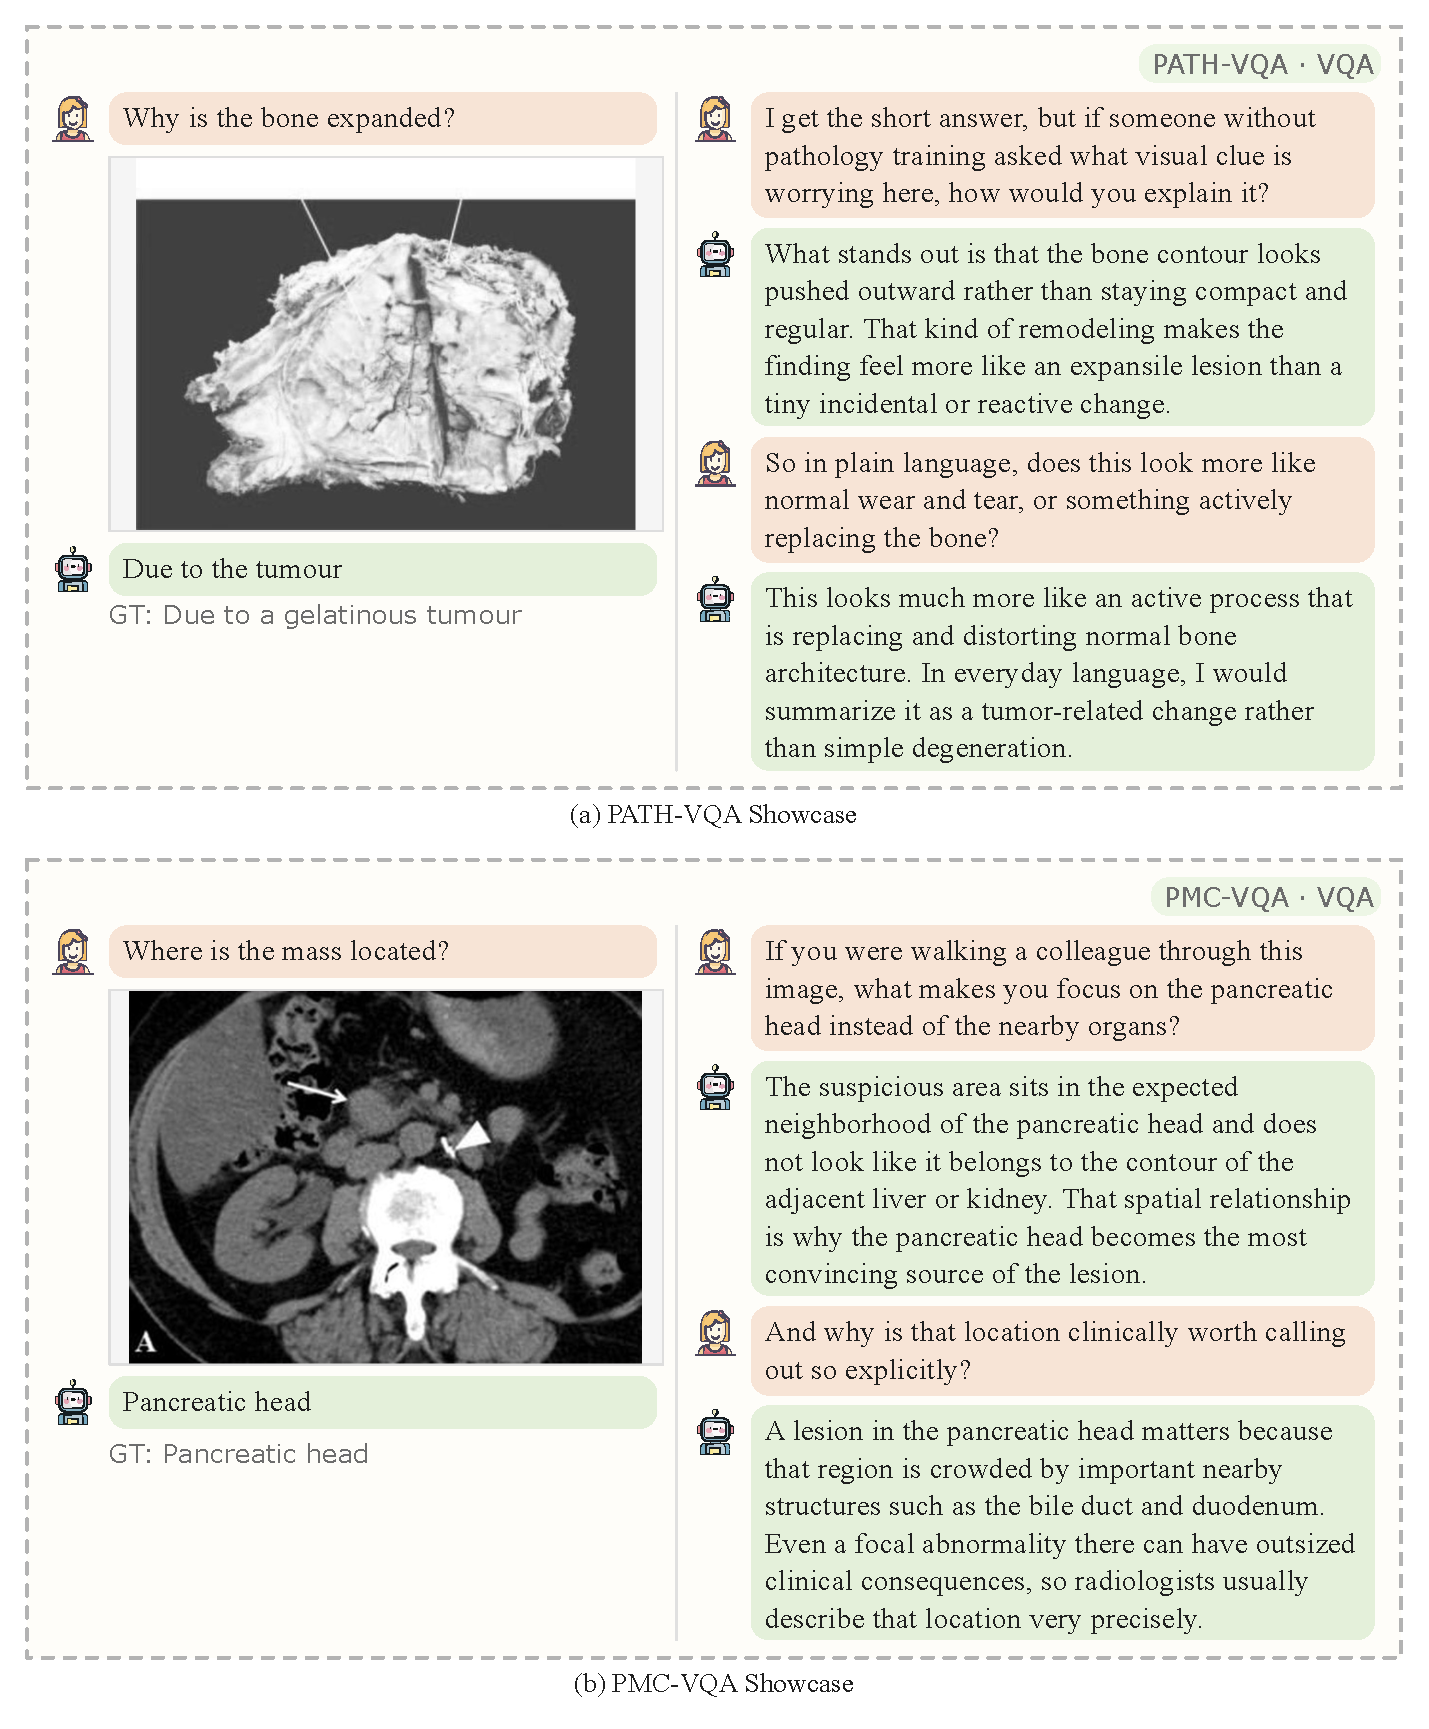
\includegraphics[width=\linewidth]{figures/showcase/medical_vqa_2d.pdf}
\caption{Multi-turn CoEvoMed dialogue examples on PathVQA (top) and PMC-VQA (bottom).}
\label{fig:showcase_path_pmc}
\end{figure}

\clearpage
\begin{figure}[H]
\centering
\includegraphics[page=2,width=\linewidth]{figures/showcase/medical_vqa_2d.pdf}
\caption{Multi-turn CoEvoMed dialogue examples on SLAKE (top) and VQA-RAD (bottom).}
\label{fig:showcase_slake_rad}
\end{figure}

\clearpage
\begin{figure}[H]
\centering
\includegraphics[page=3,width=\linewidth]{figures/showcase/medical_vqa_2d.pdf}
\caption{Multi-turn CoEvoMed dialogue examples for report generation on IU-Xray (top) and MIMIC-CXR (bottom).}
\label{fig:showcase_reports}
\end{figure}

\clearpage
\begin{figure}[H]
\centering
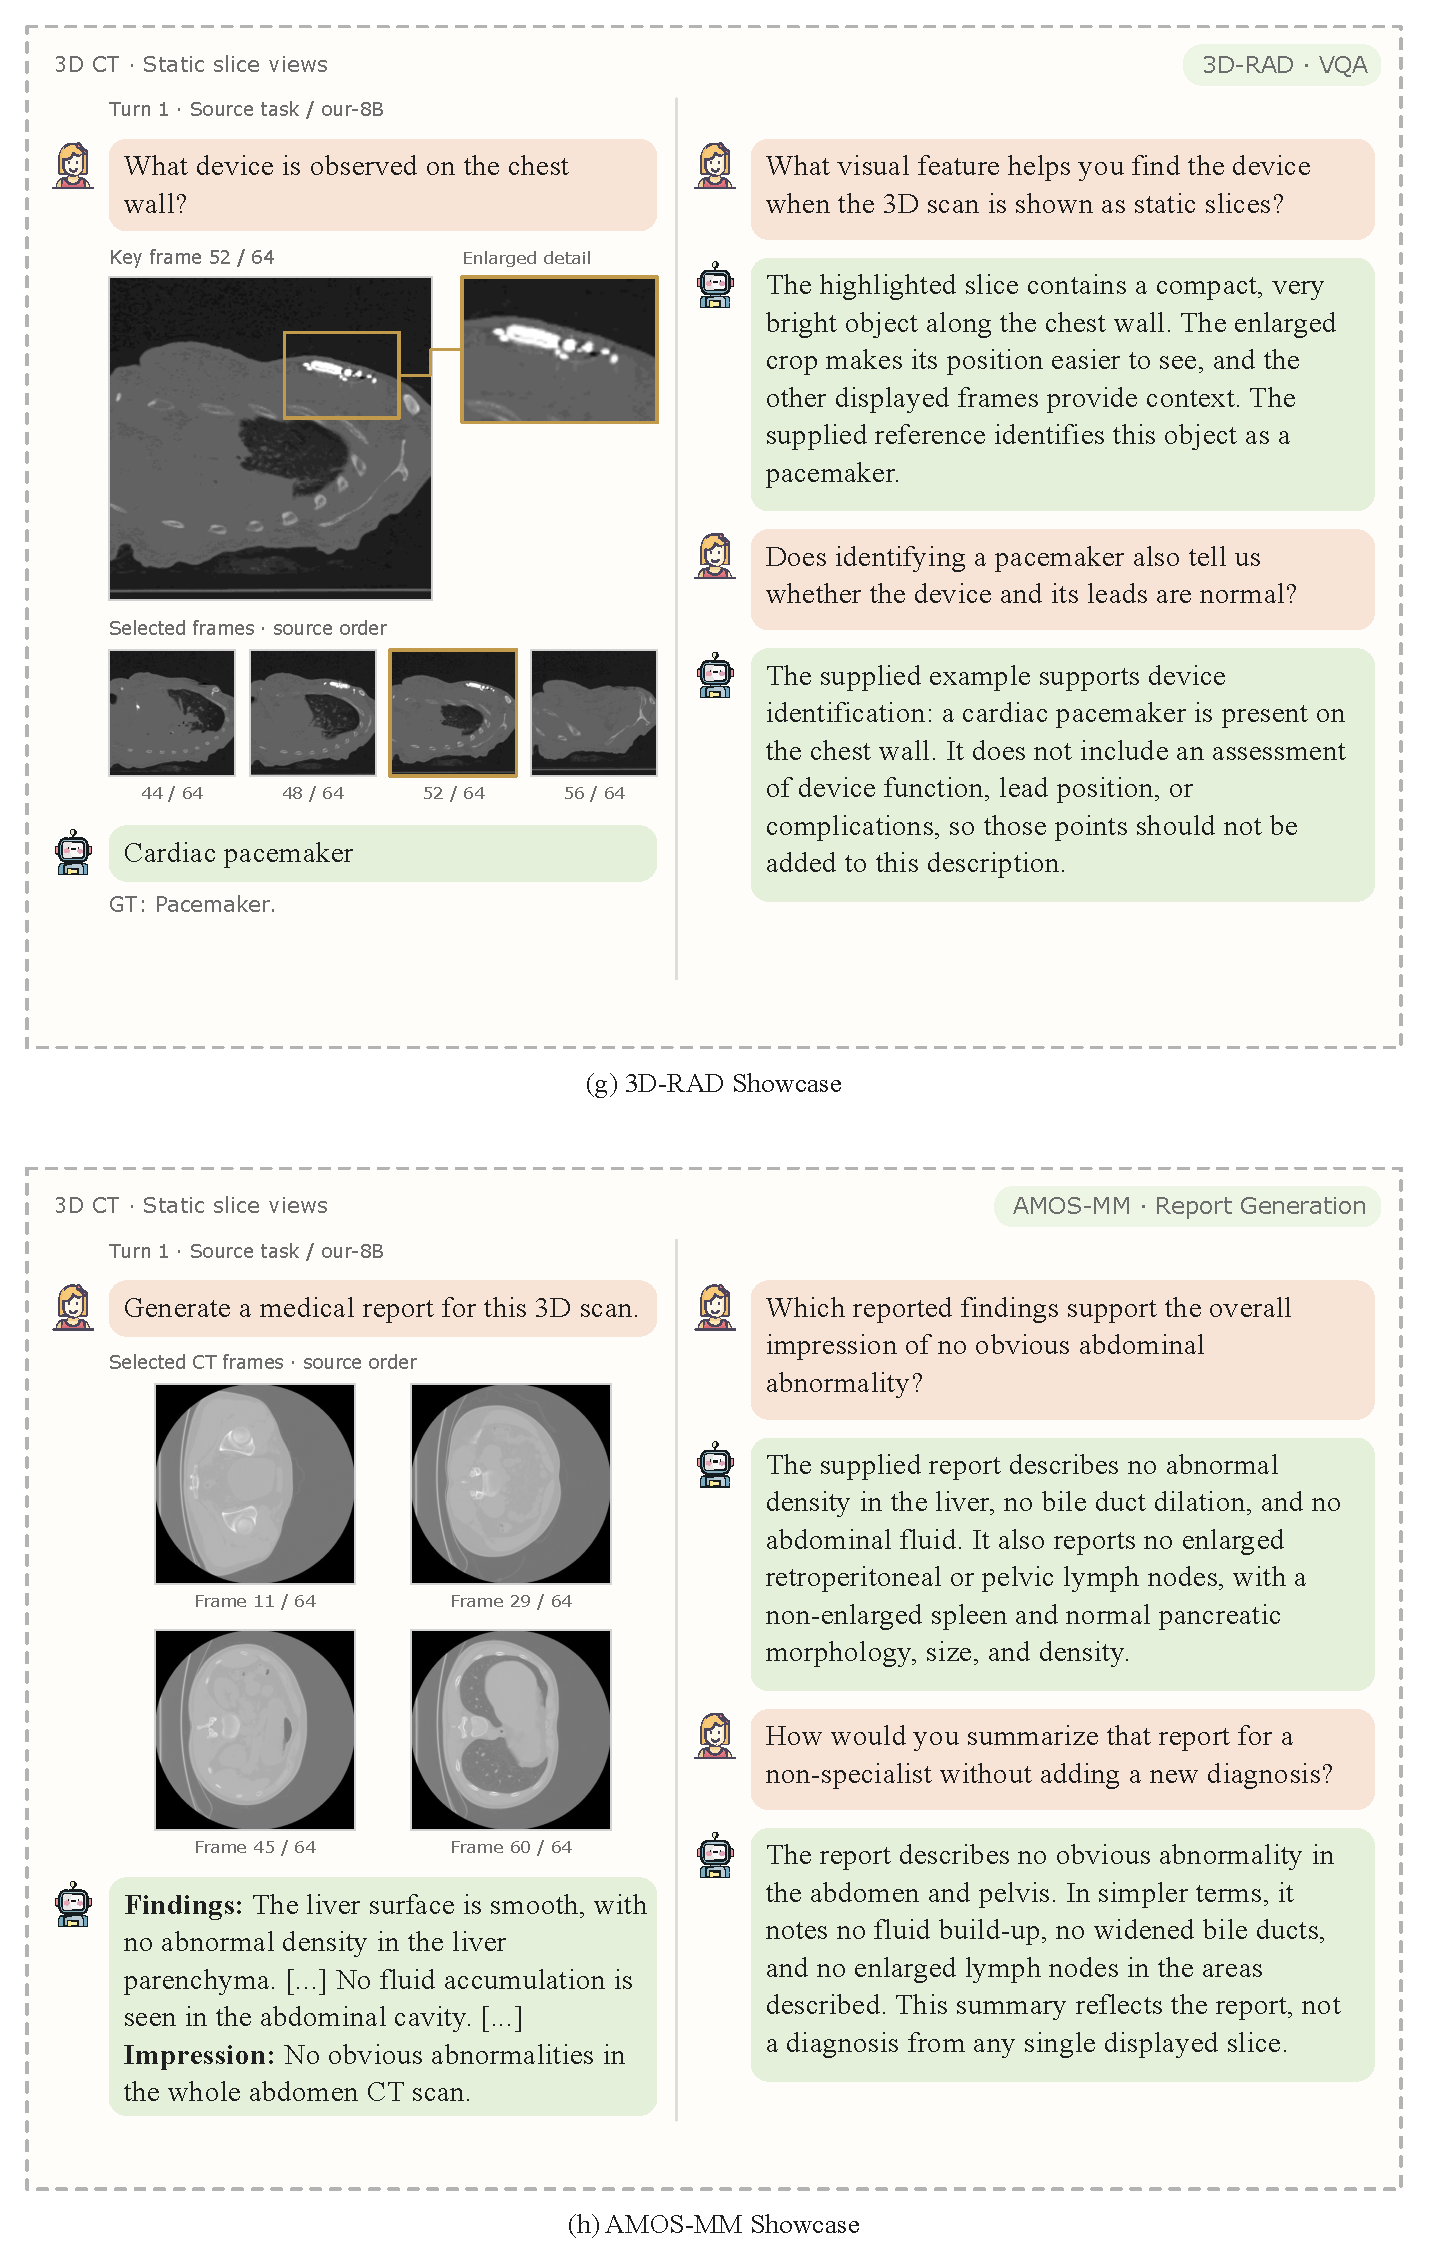
\includegraphics[width=\linewidth,height=0.86\textheight,keepaspectratio]{figures/showcase/medical_vqa_3d_pairs.pdf}
\caption{Multi-turn CoEvoMed dialogue examples on 3D-RAD (top) and AMOS-MM (bottom), with selected CT slices. The AMOS-MM report is excerpted for display; ellipses mark omitted text.}
\label{fig:showcase_rad_amos}
\end{figure}

\clearpage
\begin{figure}[H]
\centering
\includegraphics[page=2,width=\linewidth]{figures/showcase/medical_vqa_3d_pairs.pdf}
\caption{A multi-turn CoEvoMed dialogue example on M3D-VQA, with selected CT slices and an enlarged detail.}
\label{fig:showcase_m3d}
\end{figure}
